\documentclass[titlepage,11pt]{article}
\usepackage[utf8]{inputenc}  % Load inputenc first
\usepackage{comment}
\usepackage{enumitem}
\usepackage{listings}
\usepackage{amsmath}
\usepackage{graphicx}
\usepackage[font=small,labelfont=bf]{caption}
\usepackage[bahasa]{babel}
\usepackage{float}
\usepackage{verbatim}
\usepackage{graphicx,tabularx,multirow}
\usepackage{xcolor}
\usepackage[onehalfspacing]{setspace}
\usepackage[
	allcolors=visigrey,
	colorlinks=true,
]{hyperref}
\usepackage[a4paper,left=2cm,right=2cm]{geometry}
\usepackage{csquotes}
% Pengaturan kutipan artikel
\usepackage[style=ieee, backend=biber]{biblatex}
%Code listing style pak akok
\definecolor{codegreen}{rgb}{0,0.6,0}
\definecolor{codegray}{rgb}{0.5,0.5,0.5}
\definecolor{codepurple}{rgb}{0.58,0,0.82}
\definecolor{backcolour}{rgb}{0.95,0.95,0.92}

% Ubah sesuai modul
% \addbibresource{P1/pustaka/pustaka.bib}
% \addbibresource{P2/pustaka/pustaka.bib}
% \addbibresource{P3/pustaka/pustaka.bib}
\addbibresource{P4/pustaka/pustaka.bib}
% \addbibresource{P5/pustaka/pustaka.bib}

\lstdefinestyle{mystyle}{
	backgroundcolor=\color{backcolour}, commentstyle=\color{codegreen},
	keywordstyle=\color{magenta},
	numberstyle=\small\color{codegray},
	stringstyle=\color{codepurple},
	basicstyle=\ttfamily\footnotesize,
	breakatwhitespace=false,         
	breaklines=true,                 
	captionpos=t,                    
	keepspaces=true,                 
	numbers=left,                    
	numbersep=5pt,                  
	showspaces=false,                
	showstringspaces=false,
	showtabs=false,           
	frame = single,
	tabsize=2
}
\lstset{style=mystyle}

\definecolor{visigrey}{rgb}{.1,.15,.15}
\geometry{top=1cm,bottom=.5cm}
\savegeometry{titlepage}
\geometry{top=2cm,bottom=2cm}
\savegeometry{main}

\def\bspace{\(\qquad\qquad\qquad\)}
\usepackage[T1]{fontenc}
\usepackage[utf8]{inputenc}
\usepackage{tgheros}
\renewcommand*\familydefault{\sfdefault}

\setcounter{tocdepth}{6}

\def\autor{Laboratorium }
\def\lab{Multimedia dan Internet of Things}
\def\departemen{Departemen Teknik Komputer}
\def\institut{Institut Teknologi Sepuluh Nopember}
\def\praktikum{Praktikum \\ Jaringan Komputer}
% Ubah Judul sesuai dengan modul
% \def\judul{Wireless}
% \def\judul{Routing Static dan Routing Dinamis (Mikrotik)}
% \def\judul{Mengelola dan Membagi Bandwith menggunakan Qos(Simple Queue)}
\def\judul{VPN(Virtual Private Network) PPTP Pada Mikrotik}
% \def\judul{Implementasi dan Konfigurasi IP Version 6}
\def\tahun{2024}
\begin{document}
% Ubah Bahasa sesuai dengan keinginan
\selectlanguage{bahasa}
\input{Cover/Header.tex}
% Pilih Modul yang akan di build
% \section{Pendahuluan}
\subsection{Latar Belakang}
Pada modul ini, kita akan membahas konfigurasi routing static dan routing dinamis pada perangkat
MikroTik. Routing merupakan proses pengiriman data antara dua atau lebih jaringan yang berbeda.
Dalam modul ini, kita akan membahas konsep dasar routing, macam-macam routing statis dan
dinamis, serta langkah-langkah untuk mengkonfigurasi kedua jenis routing ini pada perangkat
MikroTik.\\\\
Sebelum memulai pembahasan routing, penting untuk memahami konsep dasar jaringan dan
subnetting. Jaringan terdiri dari sejumlah perangkat yang terhubung satu sama lain, seperti komputer,
printer, dan perangkat jaringan lainnya. Setiap perangkat dalam jaringan memiliki alamat IP yang
unik.

\subsection{Maksud dan Tujuan}
Mengetahui dan memahami konfigurasi routing static dan routing dinamis pada Mikrotik.

\subsection{Hasil yang diharapkan}
Dapat mengkonfigurasi konfigurasi routing static dan routing dinamis pada Mikrotik dengan
tepat.

%===========================================================%
\section{Tugas Pendahuluan}
\begin{enumerate}
\item Buatlah

%===========================================================%
\section{Alat dan Bahan}
\begin{itemize}[label=$\bullet$, itemsep=-1pt, leftmargin=*]
	\item Buatlah
\end{itemize}

%===========================================================%
\section{Jangka Waktu Pelaksanaan}
Pemahaman dan konfigurasi 1 jam.

%===========================================================%

\section{Proses dan Tahapan Konfigurasi}
%======================PERCOBAAN 1==========================%
\subsection{Wireless Point to Point}
\begin{center}

\textbf{Konfigurasi Router 1}
\begin{enumerate}
	\item Buka aplikasi WinBox pada PC 1 dan lakukan koneksi ke Router 1.\\Neighbors > Refresh > Double click Router yang terdeteksi > Connect
	      \begin{figure}[H]
		      \centering
		      \includegraphics[width=0.8\linewidth]{P1/img/per1/pc1/Step 1.png}
		      \caption{Step 1}
		      \label{fig:Step 1(Per.1 PC1)}
	      \end{figure}
\end{enumerate}

\textbf{Konfigurasi Router 2}
\begin{enumerate}
	\item Buka WinBox dan lakukan koneksi ke Router
	      \begin{figure}[H]
		      \centering
		      \includegraphics[width=0.9\linewidth]{P1/img/per1/pc2/Step 2.png}
		      \caption{Step 2}
		      \label{fig:Step 2(Per.1 PC2)}
	      \end{figure}
\end{enumerate}

\textbf{Pengujian konfigurasi}
\begin{enumerate}
\item Lakukan test ping dari Router 1 ke Router 2
\begin{figure}[H]
	\centering
	\includegraphics[width=0.9\linewidth]{P1/img/per1/pc1/Step 4.png}
	\caption{Step 1}
	\label{fig:Ping Step 1(Per.1 PC1)}
\end{figure}
\end{center}

%======================PERCOBAAN 2==========================%
\subsection{Wireless Point to Multipoint}
\begin{center}

	\textbf{Konfigurasi Router 1}
	\begin{enumerate}
		\item Berikan IP address sesuai dengan cara pengaturan IP address yang benar. Berikan IP address yang berbeda dengan contoh di modul.
		      \begin{figure}[H]
			      \centering
			      \includegraphics[width=0.9\linewidth]{P1/img/per1/pc1/Step 2.2.png}
			      \caption{Step 1}
			      \label{fig:Step 1(Per.2 PC1)}
		      \end{figure}
	\end{enumerate}

	\textbf{Konfigurasi Router 2}
	\begin{enumerate}
		\item Berikan IP address pada interface wlan 1 yang dapat dibuat pada tab IP > Addresses. Berikan IP address sesuai dengan cara pengaturan IP address yang benar. Berikan IP address yang berbeda dengan contoh di modul.
		      \begin{figure}[H]
			      \centering
			      \includegraphics[width=0.9\linewidth]{P1/img/per1/pc2/Step 2.png}
			      \caption{Step 1}
			      \label{fig:Step 1(Per.2 PC2)}
		      \end{figure}
	\end{enumerate}

	\textbf{Pengujian konfigurasi}
	\begin{enumerate}
		\item Lakukan test ping dari Router 1 ke Router 2
		      \begin{figure}[H]
			      \centering
			      \includegraphics[width=0.9\linewidth]{P1/img/per2/pc1/Step 4.png}
			      \caption{Step 1}
			      \label{fig:Ping Step 1(Per.2 PC1)}
		      \end{figure}
	\end{enumerate}

\end{center}

%======================PERCOBAAN 3==========================%
\subsection{Wireless Bridge}
\begin{center}

	\textbf{Konfigurasi Router 1}
	\begin{enumerate}
		\item Buka WinBox dan lakukan koneksi ke Router
		      \begin{figure}[H]
			      \centering
			      \includegraphics[width=0.9\linewidth]{P1/img/per3/pc1/Step 2.png}
			      \caption{Step 2}
			      \label{fig:Step 2(Per.3 PC1)}
		      \end{figure}
	\end{enumerate}

	\textbf{Konfigurasi Router 2}
	\begin{enumerate}
		\item Berikan IP address pada interface wlan1 dan ethernet 2 yang dapat dibuat pada tab IP > Addresses. Berikan IP address sesuai dengan cara pengaturan IP address yang benar. Berikan IP address yang berbeda dengan contoh di modul.
		      \begin{figure}[H]
			      \centering
			      \includegraphics[width=0.9\linewidth]{P1/img/per3/pc2/Step 2.png}
			      \caption{Step 2}
			      \label{fig:Step 2(Per.3 PC2)}
		      \end{figure}
	\end{enumerate}

	\textbf{Pengujian konfigurasi}
	\begin{enumerate}
		\item Lakukan test ping dari PC 1 ke PC 2
		      \begin{figure}[H]
			      \centering
			      \includegraphics[width=0.9\linewidth]{P1/img/per3/pc1/Step 7.png}
			      \caption{Step 7}
			      \label{fig:Step 7(Per.3 PC1)}
		      \end{figure}
	\end{enumerate}

\end{center}

%===========================================================%
\section{Hasil yang didapat}
Memahami dan mengkonfigurasi koneksi Point to Point, Point to Multipoint dan Wireless
Bridging dengan tepat.

%===========================================================%
\section{Temuan Permasalahan}
Firewall hidup pada Laptop dapat mempengaruhi koneksi wireless tidak terhubung, kalian
bisa menonaktifkan firewall di laptop kalian, tetapi hal ini tidak terjadi di semua perangkat.

%===========================================================%
\section{Kesimpulan}
Dengan memahami dan mengkonfigurasi 3 jenis koneksi pada wireless, kita dapat
mengimplementasikan koneksi wireless dengan tepat sesuai kebutuhan dan kondisi tertentu.

% \input{P2/RoutingStatisdanDinamis.tex}
% \input{P3/ManajemenBandwith.tex}
\input{P4/VPN.tex}
% \section{Pendahuluan}
\subsection{Latar Belakang}
Internet Protocol Address v6 (IPv6) adalah standar protokol yang digunakan untuk mengidentifikasi dan
mengarahkan alamat jaringan dalam jaringan komputer. Dibandingkan dengan pendahulunya, IPv4, IPv6
memiliki format alamat yang lebih panjang dengan 128 bit, yang memungkinkan jumlah alamat yang jauh
lebih besar, sehingga dapat mengatasi kekurangan alamat IPv4 yang semakin berkurang. IPv6 juga
mendukung fitur-fitur tambahan, termasuk pemantauan aliran lalu lintas, keamanan yang ditingkatkan, dan
kualitas layanan yang lebih baik, menjadikannya solusi jangka panjang untuk pertumbuhan Internet yang
pesat dan kebutuhan alamat yang terus berkembang.

\subsection{Maksud dan Tujuan}
\begin{center}
    \begin{enumerate}
        \item Mengetahui bagaimana konfigurasi static routing menggunakan Ipv6
        \item Mengimplementasikan konfigurasi Ipv6 pada perangkat mikrotik
    \end{enumerate}
\end{center}

%===========================================================%
\section{Tugas Pendahuluan}
\begin{center}
	\colorbox{cyan!30}{\parbox{0.8\linewidth}{
    \begin{enumerate}
        \item Apa solusi lain ketika IPv4 habis, selain menggunakan IPv6?
        \item Sebutkan tiga keunggulan IPv6 dibandingkan IPv4!
        \item Mengapa panjang awal alamat IPv6 biasanya adalah 128 bit?
    \end{enumerate}}}
\end{center}

%===========================================================%
\section{Alat dan Bahan}
\begin{itemize}[label=$\bullet$, itemsep=-1pt, leftmargin=*]
	\item 2 buah Cloud Core Router
	\item 3 Kabel UTP (LAN)
	\item 2 buah Laptop
	\item Software Winbox
\end{itemize}

%===========================================================%
\section{Jangka Waktu Pelaksanaan}
Pemahaman dan konfigurasi 1 jam.

%===========================================================%
\section{Penjelasan dan Tahapan Konfigurasi}

%======================PERCOBAAN 1==========================%
\begin{center}
    \textbf{Konfigurasi PC 1}
    \begin{enumerate}

        \item Buka aplikasi Winbox pada PC1 dan hubungkan ke Router. Pastikan Login terisi “admin”, Klik Neighbors > Klik Refresh > Pilih Router yang ingin disambungkan > Klik Connect.
        \begin{figure}[H]
			\centering
			\includegraphics[width=0.5\linewidth]{P5/img/pc1/Step 1.png}
			\caption{Step 1}
			\label{fig:Step 1(PC 1)}
		\end{figure}

        \item Konfigurasikan Router1 untuk mengaktifkan layanan IPv6. Klik System > Klik Packages > Klik IPv6 > Klik Enable > Reboot ulang Router1.
        \begin{figure}[H]
			\centering
			\includegraphics[width=0.5\linewidth]{P5/img/pc1/Step 2.png}
			\caption{Step 2}
			\label{fig:Step 2(PC 1)}
        \end{figure}

        \item Konfigurasi IPv6 Router 1 untuk menghubungkan PC 1 dengan Router 1. Tambahkan IP address > Isi address > pilih Interface yang terhubung ke PC 1 atau ether4 > Klik Apply > Klik OK.
        \begin{figure}[H]
			\centering
			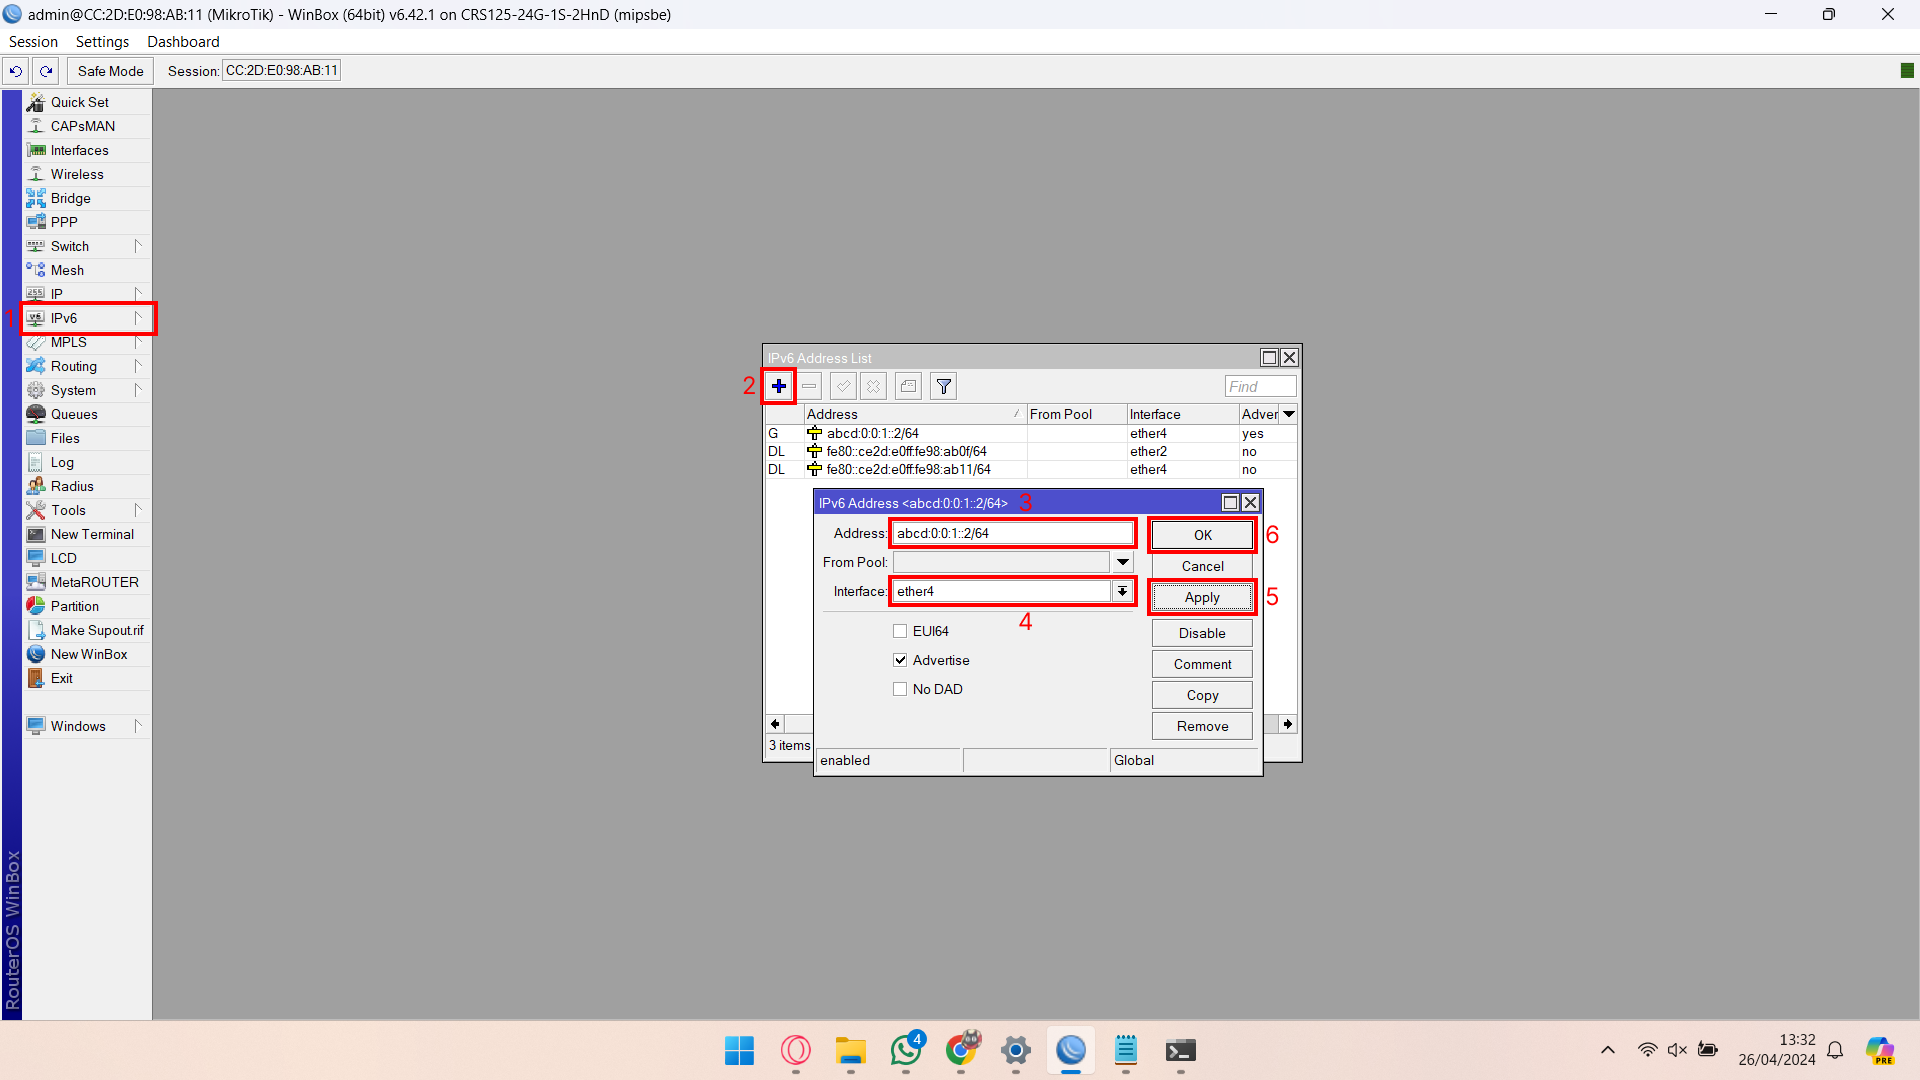
\includegraphics[width=0.8\linewidth]{P5/img/pc1/Step 3.png}
			\caption{Step 3}
			\label{fig:Step 3(PC 1)}
		\end{figure}

        \item Konfigurasi IPv6 pada PC 1 dengan mengubah pengaturan pada setting ethernet. Ubah IPv6 perangkat yang otomatis menjadi manual, pastikan IPv6 PC 1 masih satu jaringan dengan IPv6 lokal yang diinginkan, isi Gateway dengan IPv6 address Router 1 yang tersambung dengan PC 1. Berikan IPv6 address yang berbeda dengan contoh yang ada di modul.
        \begin{figure}[H]
			\centering
			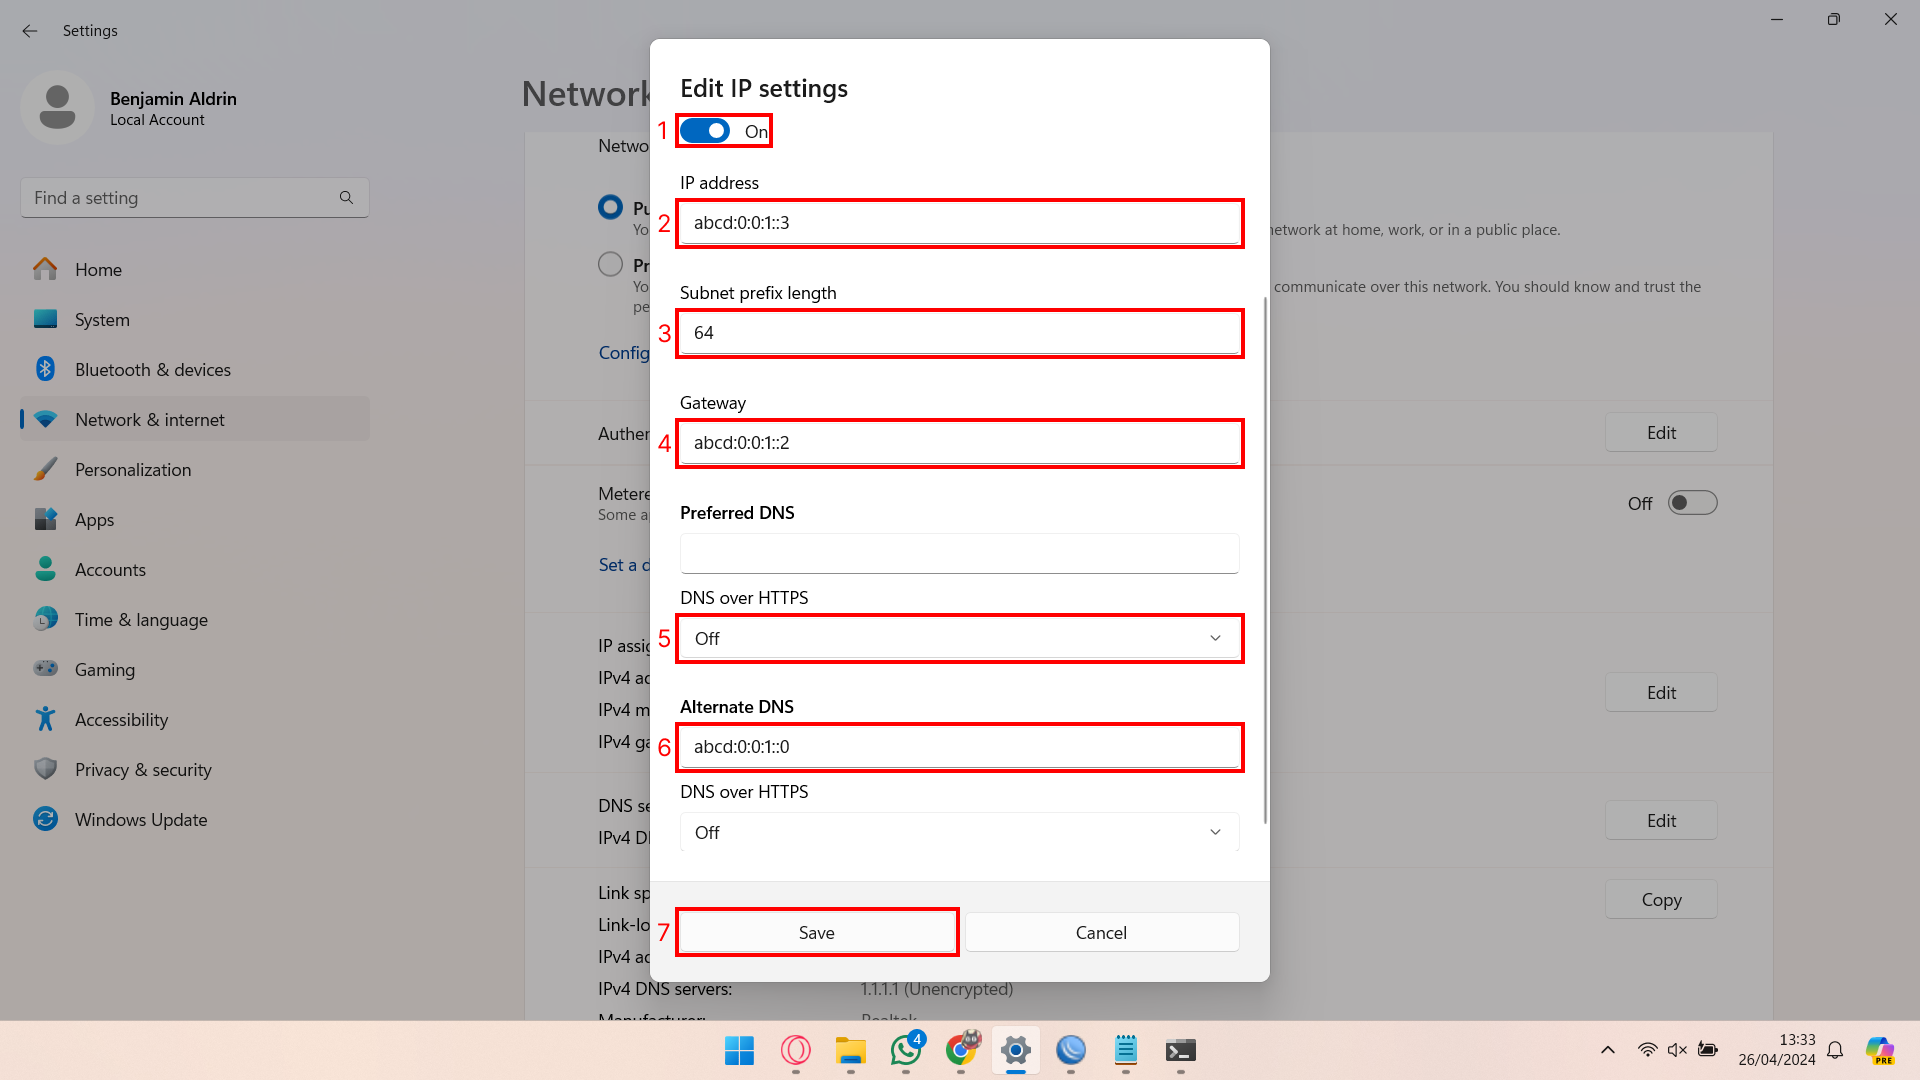
\includegraphics[width=0.8\linewidth]{P5/img/pc1/Step 4.png}
			\caption{Step 4}
			\label{fig:Step 4(PC 1)}
		\end{figure}

        \item Lakukan uji coba ping dari Router 1 ke PC 1 dan sebaliknya untuk memastikan kedua perangkat sudah saling terhubung.
        \begin{figure}[H]
			\centering
			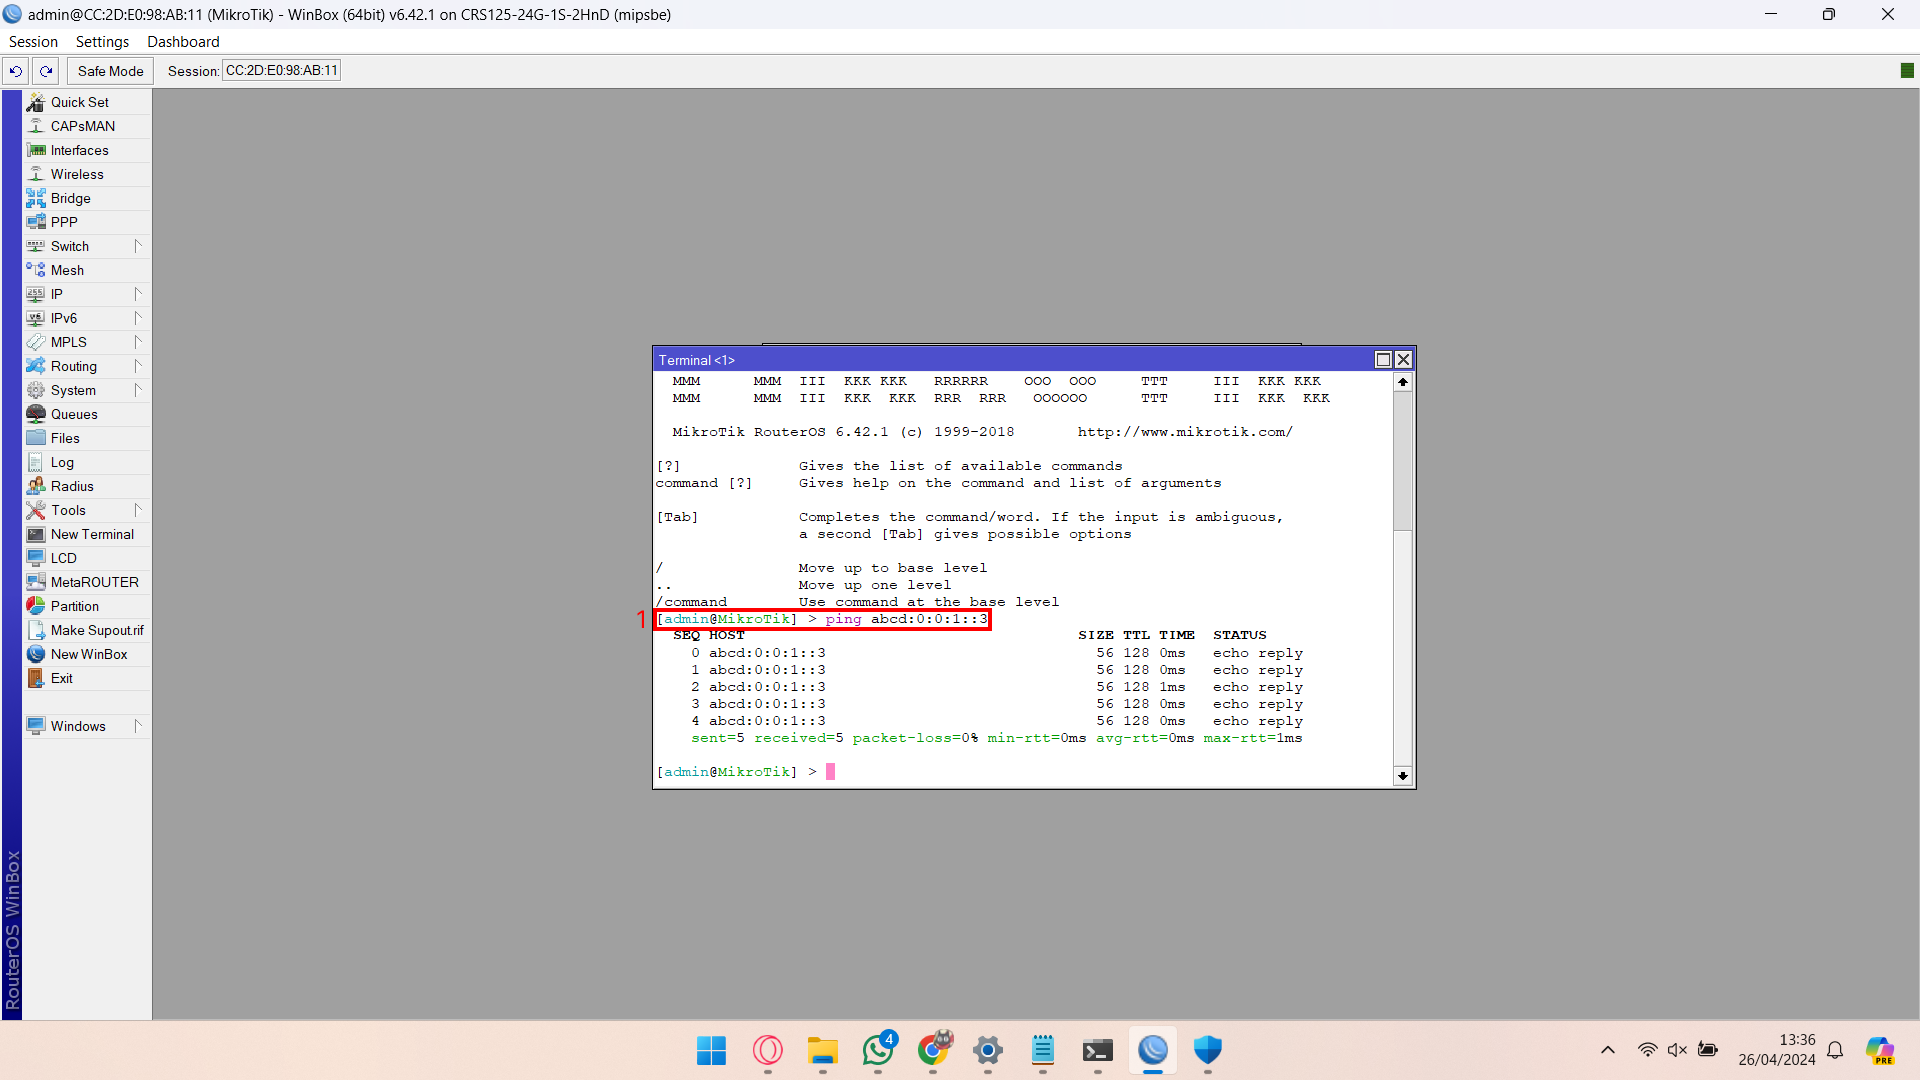
\includegraphics[width=0.8\linewidth]{P5/img/pc1/Step 5.png}
			\caption{Step 5}
			\label{fig:Step 5(PC 1)}
		\end{figure}

        \item Konfigurasi IPv6 Router 1 untuk menghubungkan Router 1 dengan Router 2. Tambahkan address IPv6 > Isi address > pilih Interface yang terhubung ke Router 2 (ether2) > Klik Apply > Klik OK.
        \begin{figure}[H]
			\centering
			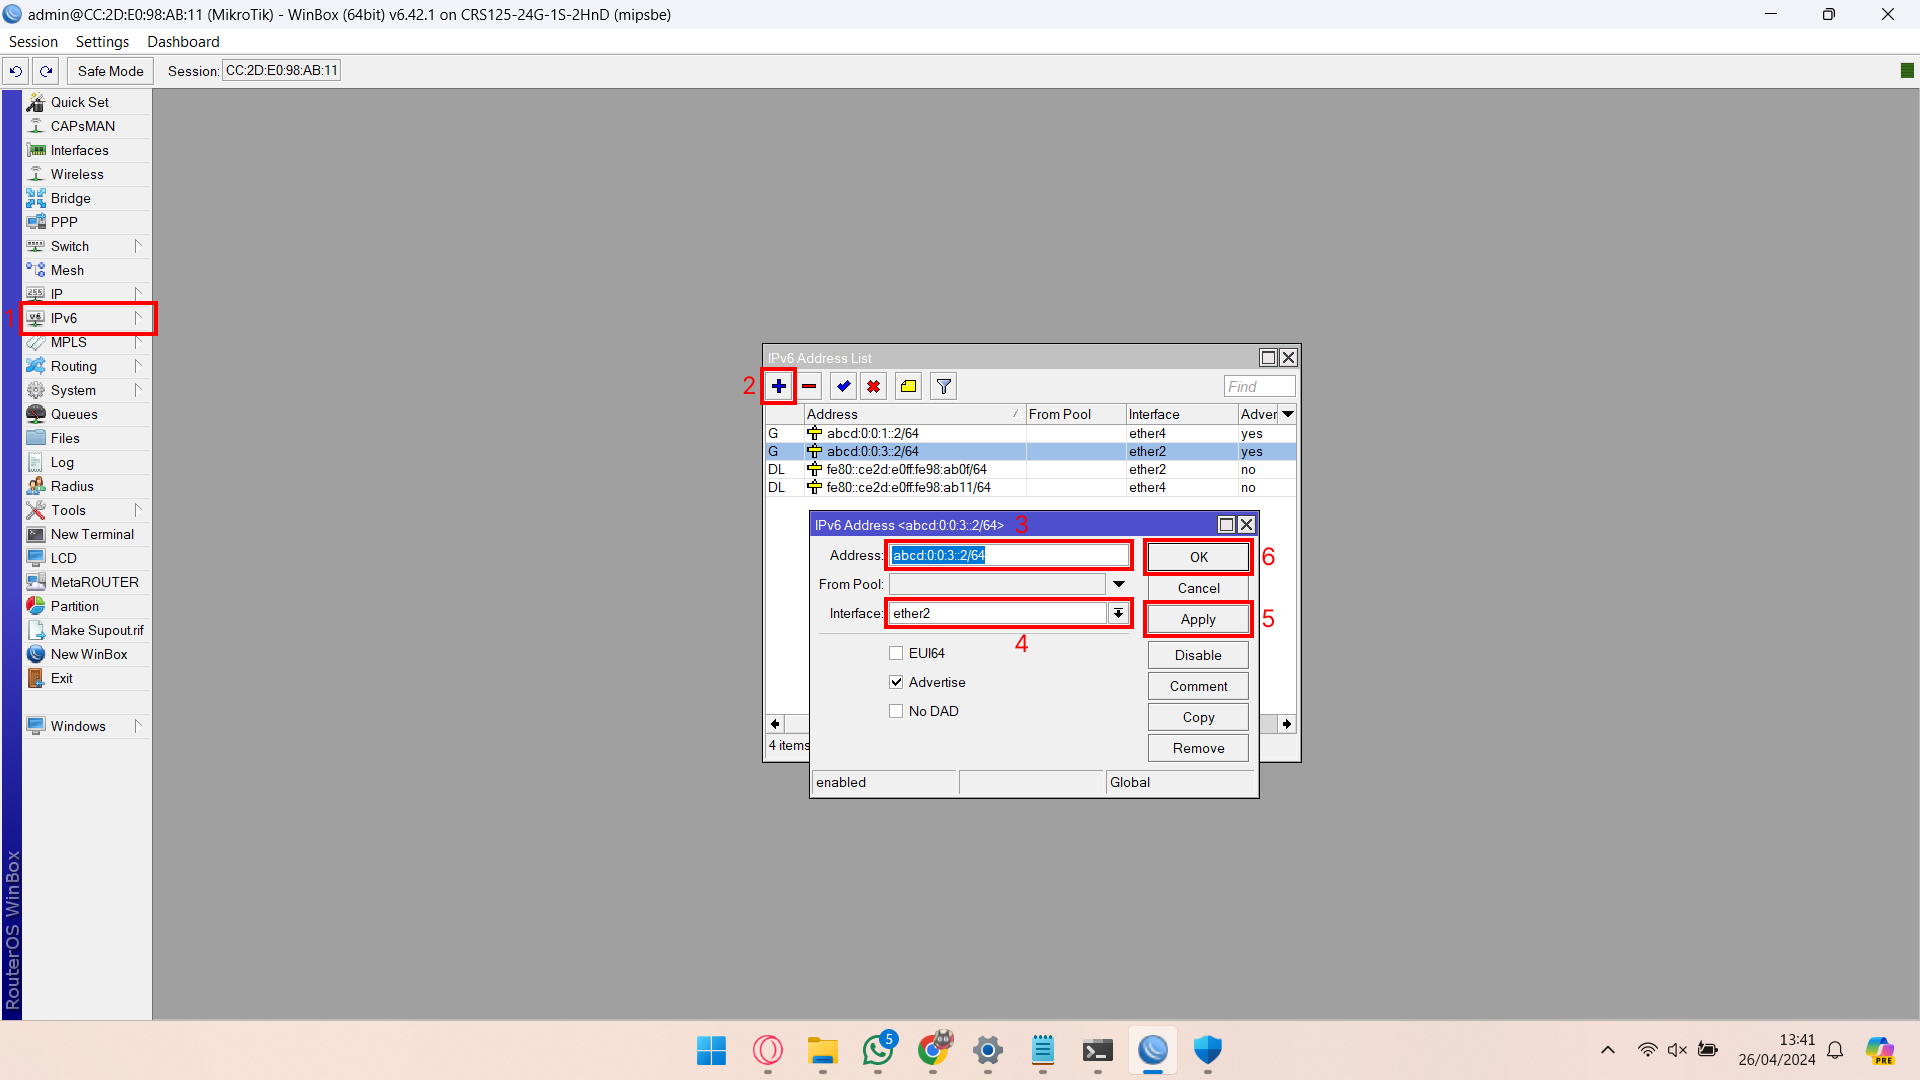
\includegraphics[width=0.8\linewidth]{P5/img/pc1/Step 6.png}
			\caption{Step 6}
			\label{fig:Step 6(PC 1)}
		\end{figure}

        \item Hubungkan kedua Network menggunakan routing statis. Buka pada tab IPv6 > Routes. Lalu tambahkan routes. Masukkan alamat jaringan yang ingin dituju, melalui alamat Gateway pada Router 2.
        \begin{figure}[H]
			\centering
			\includegraphics[width=0.8\linewidth]{P5/img/pc1/Step 7.png}
			\caption{Step 7}
			\label{fig:Step 7(PC 1)}
		\end{figure}
    \end{enumerate}

    \textbf{Konfigurasi PC 2}
    \begin{enumerate}
        \item Buka aplikasi Winbox pada PC2 dan hubungkan ke Router. Pastikan Login terisi “admin”, Klik Neighbors > Klik Refresh > Pilih Router yang ingin disambungkan > Klik Connect.
        \begin{figure}[H]
			\centering
			\includegraphics[width=0.5\linewidth]{P5/img/pc2/Step 1.png}
			\caption{Step 1}
			\label{fig:Step 1(PC 2)}
		\end{figure}
        \item Konfigurasikan Router2 untuk mengaktifkan layanan IPv6. Klik System > Klik Packages > Klik IPv6 > Klik Enable > Reboot ulang Router2.
        \begin{figure}[H]
			\centering
			\includegraphics[width=0.5\linewidth]{P5/img/pc2/Step 2.png}
			\caption{Step 2}
			\label{fig:Step 2(PC 2)}
        \end{figure}
        \item Konfigurasi IPv6 Router 2 untuk menghubungkan PC 2 dengan Router 2. Tambahkan IP address > Isi address > pilih Interface yang terhubung ke PC 2 (ether4) > Klik Apply > Klik OK.
        \begin{figure}[H]
			\centering
			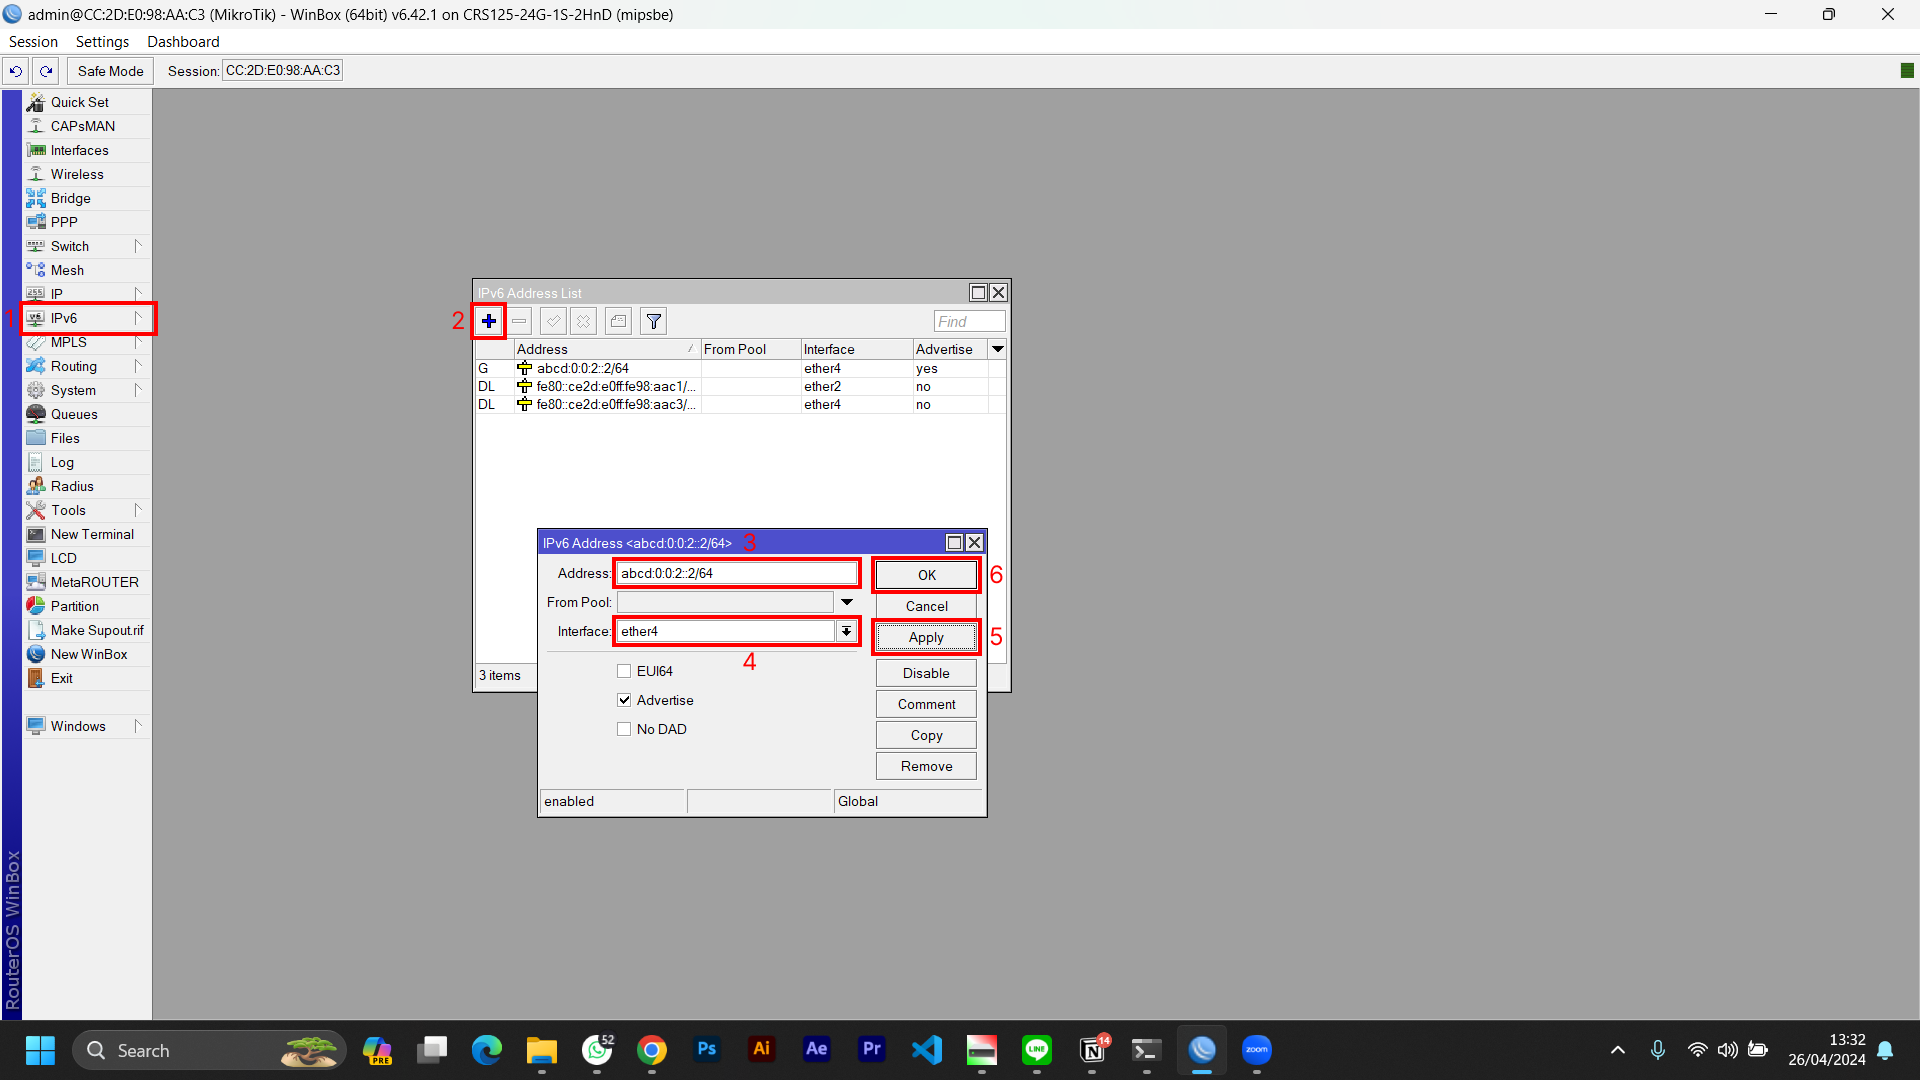
\includegraphics[width=0.8\linewidth]{P5/img/pc2/Step 3.png}
			\caption{Step 3}
			\label{fig:Step 3(PC 2)}
		\end{figure}
        \item Konfigurasi IPv6 pada PC 2 dengan mengubah pengaturan pada setting ethernet. Ubah IPv6 perangkat yang otomatis menjadi manual, pastikan IPv6 PC 2 masih satu jaringan dengan IPv6 lokal yang diinginkan, isi Gateway dengan IPv6 address Router 2 yang tersambung dengan PC 2. Berikan IPv6 address yang berbeda dengan contoh yang ada di modul.
        \begin{figure}[H]
			\centering
			\includegraphics[width=0.8\linewidth]{P5/img/pc2/Step 4.png}
			\caption{Step 4}
			\label{fig:Step 4(PC 2)}
		\end{figure}
        \item Lakukan uji coba ping dari Router 2 ke PC 2 dan sebaliknya untuk memastikan kedua perangkat sudah saling terhubung.
        \begin{figure}[H]
			\centering
			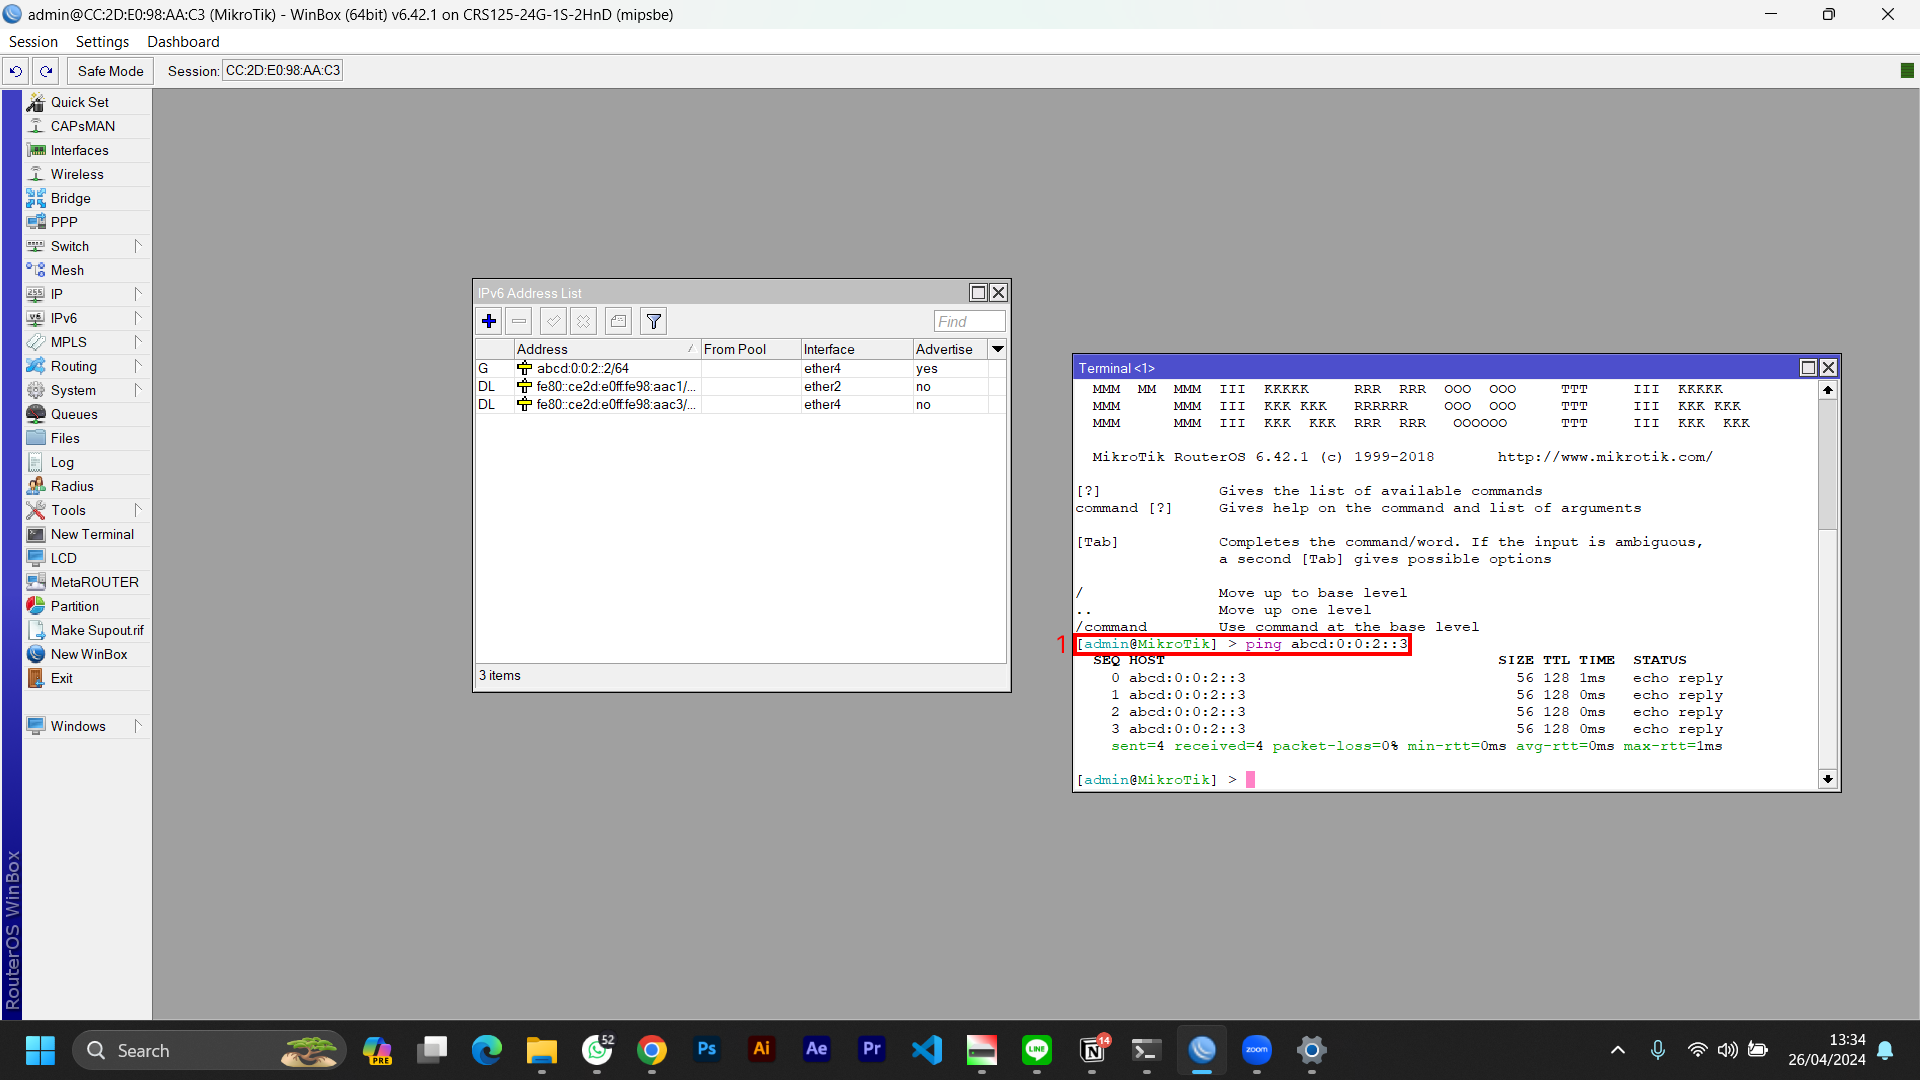
\includegraphics[width=0.8\linewidth]{P5/img/pc2/Step 5.png}
			\caption{Step 5}
			\label{fig:Step 5(PC 2)}
		\end{figure}
    
        \item Konfigurasi IPv6 Router 2 untuk menghubungkan Router 2 dengan Router 1. Tambahkan address IPv6 > Isi address > pilih Interface yang terhubung ke Router 1 (ether2) > Klik Apply > Klik OK.
        \begin{figure}[H]
			\centering
			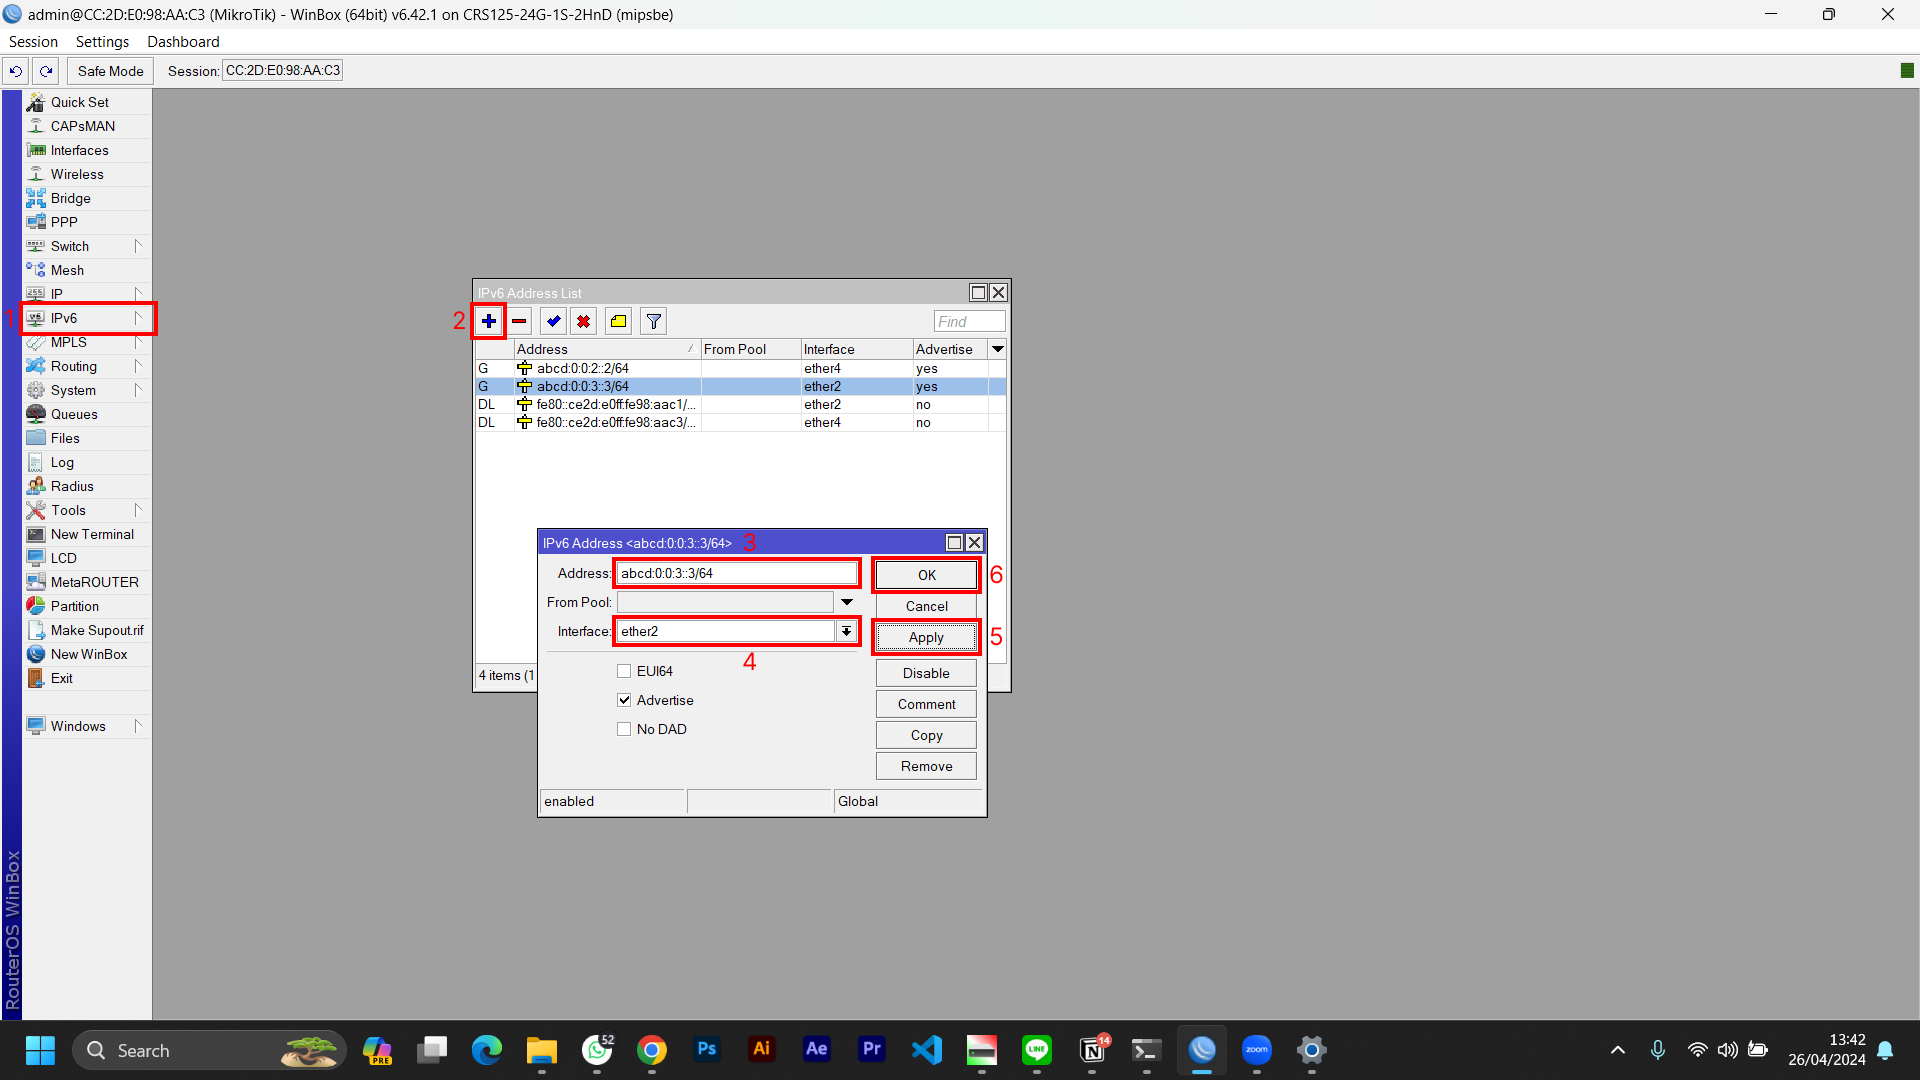
\includegraphics[width=0.8\linewidth]{P5/img/pc2/Step 6.png}
			\caption{Step 6}
			\label{fig:Step 6(PC 2)}
		\end{figure}
        \item Hubungkan kedua Network menggunakan routing statis. Buka pada tab IPv6 > Routes. Lalu tambahkan routes. Masukkan alamat jaringan yang ingin dituju, melalui alamat Gateway pada Router 1.
        \begin{figure}[H]
			\centering
			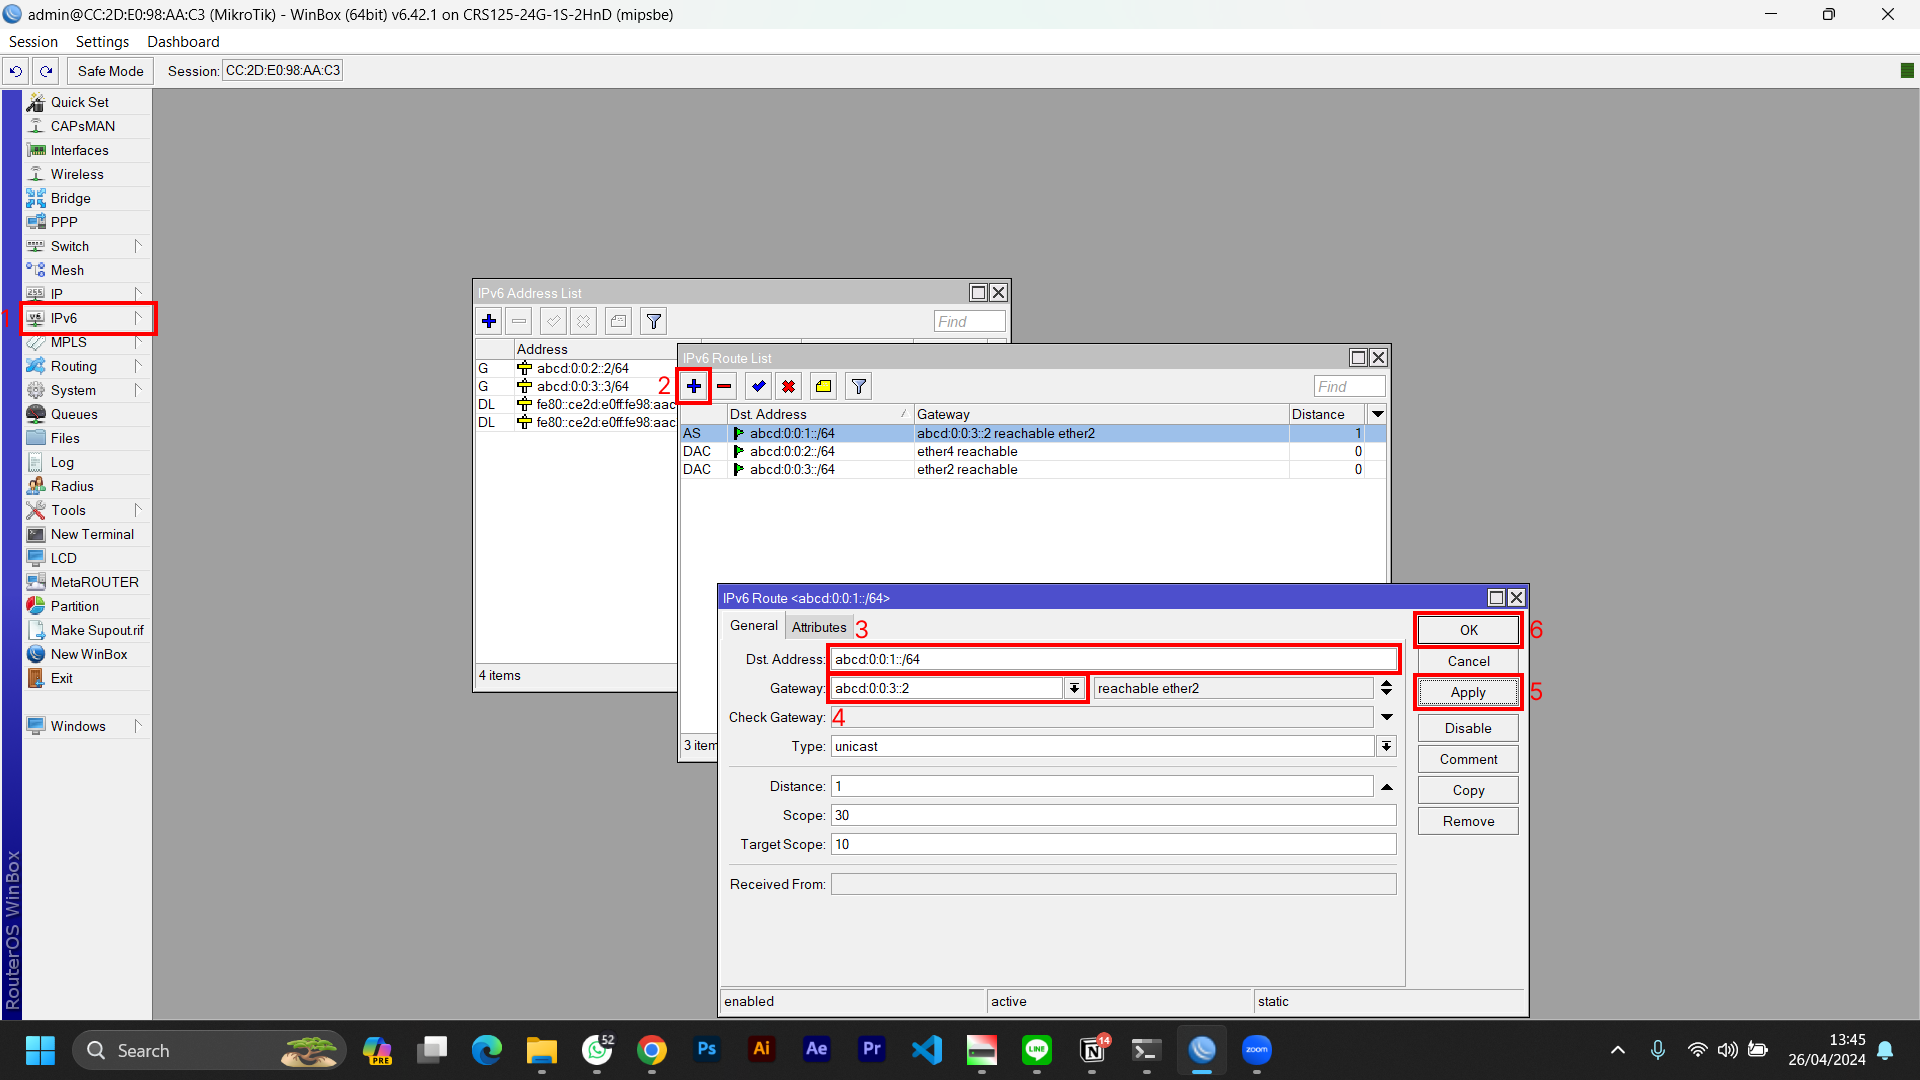
\includegraphics[width=0.8\linewidth]{P5/img/pc2/Step 7.png}
			\caption{Step 7}
			\label{fig:Step 7(PC 2)}
		\end{figure}
    \end{enumerate}

	\textbf{Pengujian Konfigurasi}
	\begin{enumerate}
		\item Lakukan tes ping ke alamat IPv6 PC 2 untuk memastikan kedua PC sudah terhubung.
		\begin{figure}[H]
			\centering
			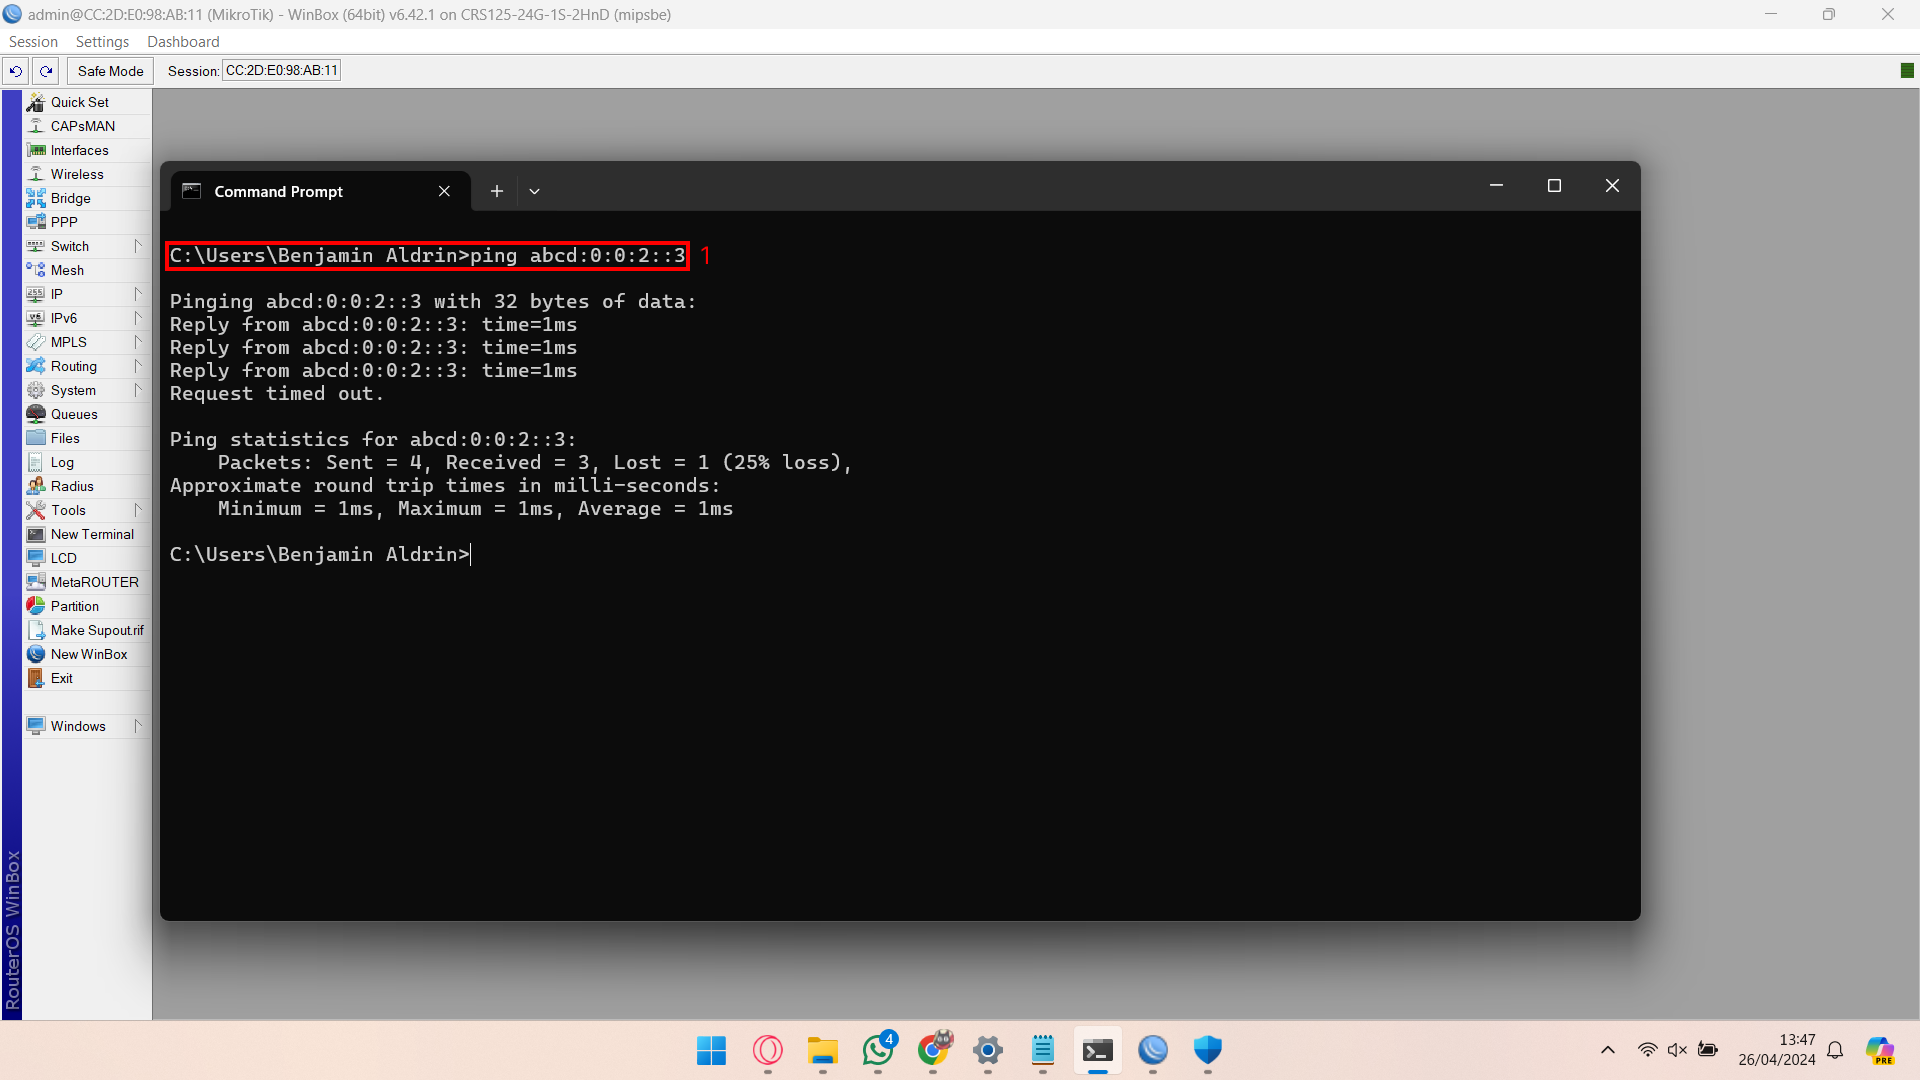
\includegraphics[width=0.8\linewidth]{P5/img/pc1/Step 8.png}
			\caption{Step 1}
			\label{fig:Ping Step 1}
		\end{figure}
        \item Lakukan tes ping ke alamat IPv6 PC 1 untuk memastikan kedua PC sudah terhubung.
		\begin{figure}[H]
			\centering
			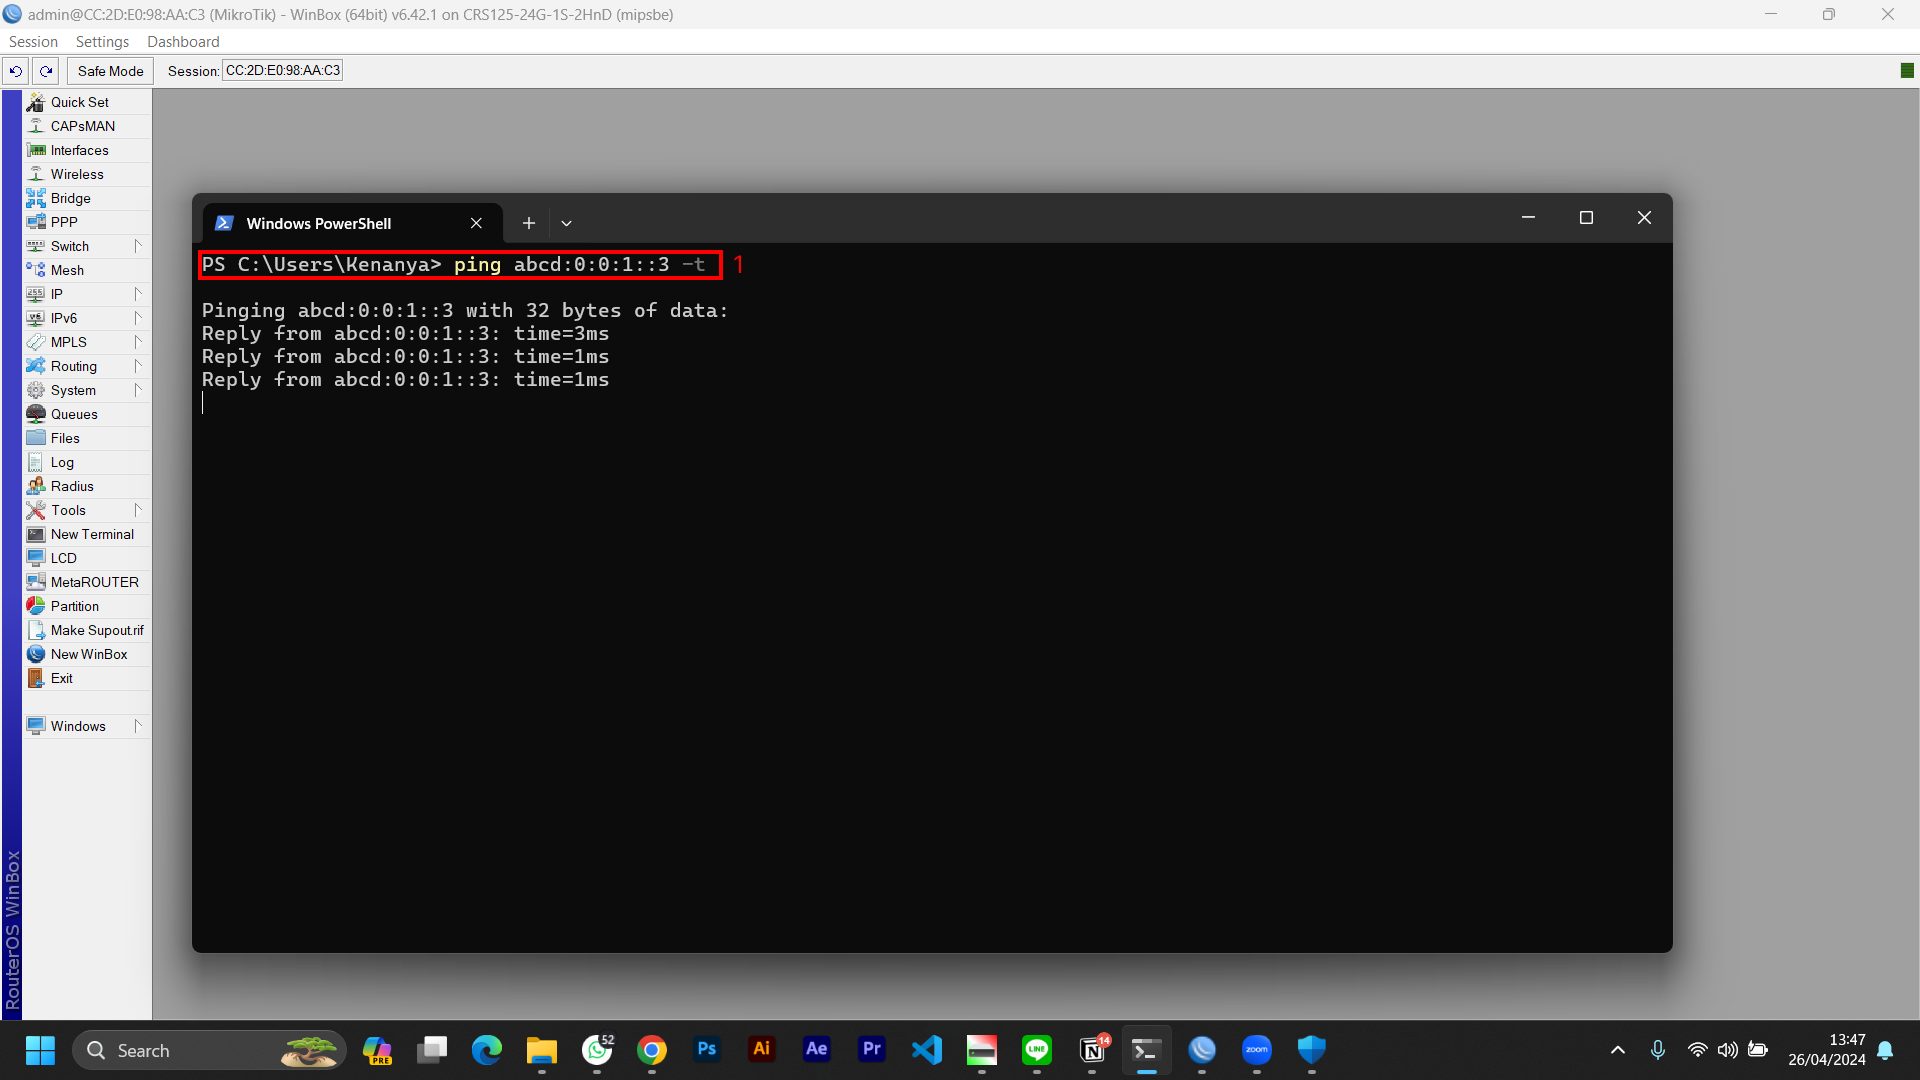
\includegraphics[width=0.8\linewidth]{P5/img/pc2/Step 8.png}
			\caption{Step 2}
			\label{fig:Ping Step 2}
		\end{figure}
	\end{enumerate}

\end{center}

%===========================================================%
\section{Hasil yang didapat}
Memahami penerapan dan penghubungan jaringan dengan menerapkan IPv6 pada konfigurasi statis

%===========================================================%
\section{Kesimpulan}
Dalam mengkonfigurasi IPv6, diperlukan pemahaman dasar mengenai penghubungan jaringan dengan menggunakan konfigurasi statis



\renewcommand\refname{Daftar Pustaka} % Menghilangkan kata "Daftar Pustaka"
\renewcommand{\bibname}{} % Menghilangkan kata "Bibliography"

\printbibliography
\end{document}